\documentclass{article}
\usepackage{tikz}

\begin{document}
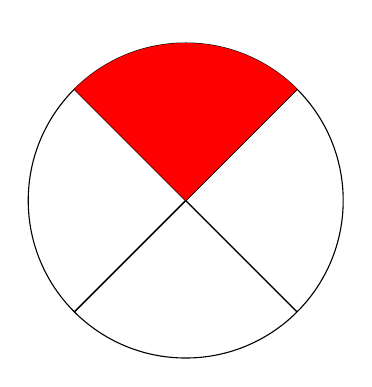
\begin{tikzpicture}
  \draw (0,0) circle (2cm); % desenha o círculo com raio de 2cm

  % desenha os diâmetros
  \draw (45:2) -- (225:2);
  \draw (135:2) -- (315:2);

  % desenha as linhas que dividem o círculo em quatro partes iguais
  \draw (0,0) -- (45:2);
  \draw (0,0) -- (135:2);
  \draw (0,0) -- (225:2);
  \draw (0,0) -- (315:2);

  \fill[red] (0,0) -- (45:2) arc (45:135:2) -- cycle;
\end{tikzpicture}
\end{document}
